%%%%%%%%%%%%%%%%%%%%%%%%%%%%%%%%%%%%%%%%%
% University/School Laboratory Report
% LaTeX Template
% Version 3.1 (25/3/14)
%
% This template has been downloaded from:
% http://www.LaTeXTemplates.com
%
% Original author:
% Linux and Unix Users Group at Virginia Tech Wiki 
% (https://vtluug.org/wiki/Example_LaTeX_chem_lab_report)
%
% License:
% CC BY-NC-SA 3.0 (http://creativecommons.org/licenses/by-nc-sa/3.0/)
%
%%%%%%%%%%%%%%%%%%%%%%%%%%%%%%%%%%%%%%%%%

%----------------------------------------------------------------------------------------
%	PACKAGES AND DOCUMENT CONFIGURATIONS
%----------------------------------------------------------------------------------------

\documentclass{article}

\usepackage[version=3]{mhchem} % Package for chemical equation typesetting
\usepackage{siunitx} % Provides the \SI{}{} and \si{} command for typesetting SI units
\usepackage{graphicx} % Required for the inclusion of images
\usepackage{natbib} % Required to change bibliography style to APA
\usepackage{amsmath} % Required for some math elements 
\usepackage{float}
\usepackage{commath}%for math abs

\setlength\parindent{0pt} % Removes all indentation from paragraphs

\renewcommand{\labelenumi}{\alph{enumi}.} % Make numbering in the enumerate environment by letter rather than number (e.g. section 6)

%\usepackage{times} % Uncomment to use the Times New Roman font

%----------------------------------------------------------------------------------------
%	DOCUMENT INFORMATION
%----------------------------------------------------------------------------------------

\title{Image Preprocessing\\Gonzalez\\Spatial Preprocessing} % Title

\author{Ahmad \textsc{Asadi}} % Author name

\date{\today} % Date for the report

\begin{document}

\maketitle % Insert the title, author and date

\begin{center}
\begin{tabular}{l r}
Date Performed: & February 21, 2016 \\ % Date the experiment was performed
%Partners: & James Smith \\ % Partner names
%& Mary Smith \\
Instructor: & Professor Safabakhsh % Instructor/supervisor
\end{tabular}
\end{center}

% If you wish to include an abstract, uncomment the lines below
% \begin{abstract}
% Abstract text
% \end{abstract}

%----------------------------------------------------------------------------------------
%	SECTION 1
%----------------------------------------------------------------------------------------

\section{Overview and Definitions}
\begin{description}
\item [Spatial Domain Process] Formally is defined as:\\
	\begin{center}$g(x,y) = T[f(x,y)]$\end{center}
	where $T$ is an operator defined over a neighbourhood of $(x,y)$ on $f$. Also it can be defined on a set of input images.
\item [Definition of Neighbourhood] 
	Usually as a \textbf{square or rectangular subimage} centered at $(x,y)$.
\item [Gray-level transformation] If neighbourhood radius is equal to 1 then $T$ is a \textbf{Gray-level}, or \textbf{Intensity} or \textbf{Mapping}, transformation function.
It is:\\
	\begin{center}$ s = T(r) $\end{center}
	where s and r are respectively the gray level of $g(x,y)$ and $f(x,y)$.\\
	\textbf{Techniques using gray-level transformation, as they operate on just a single point, are mostly referred to as \textit{point processing}.}
\item [Mask] Masks or filters are 2D arrays with a specific size in which inner weights define the application and effect of the mask.
\end{description}

%------------------------------------------------------------------------------------
\section{Some Basic Gray-level Transformations}
 \begin{description}
 \item [Negative Image] A negative image of an input image with gray levels in the range [0 , L-1] is defined as:\\
 \begin{center}
 $s = (L-1) - r$
 \end{center}
 Following is an example of application:
 \begin{figure}
 \center
\makebox[\textwidth]{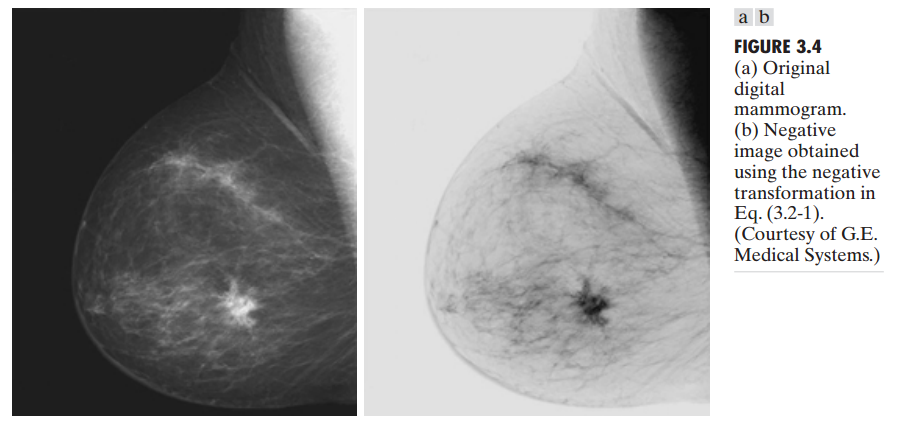
\includegraphics[width=300px]{./Imgs/neg.png}}
\caption{This figure illustrates evident contribution of reversing the intensity (negating image) to illustrate existence of lesion in a part of body.}
 \end{figure}
 
 \item [Log Transformation] The general form of this transformation is as follows:\\
 \begin{center}
 $s = c \log^{(1+r)}$
 \end{center}
 This transformation maps a narrow range of low gray-levels in input image to a wider range in output.\\
 This transformation is appropriate for applications in which having more details of darker parts of image along with bright parts makes worthwhile contributions to accomplish the required task.
 \begin{figure}
 \center
 \makebox[\textwidth]{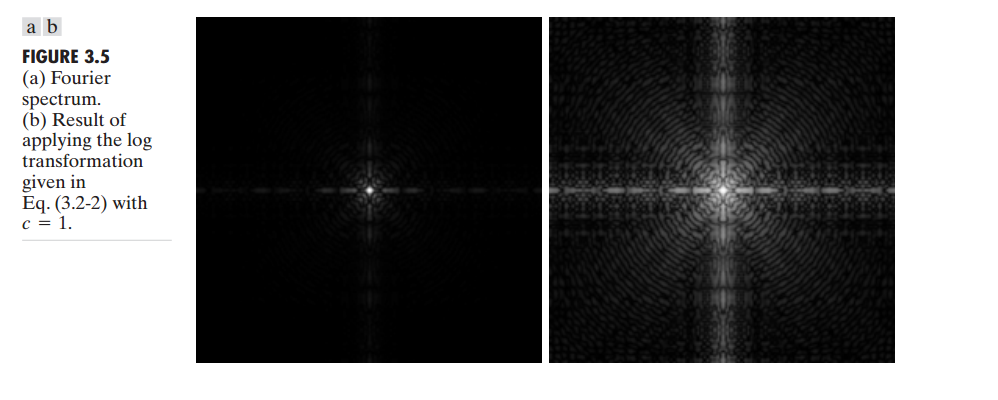
\includegraphics[width=300px]{./Imgs/log.png}}
 \caption{Log transformation effect on input picture}
 \end{figure}
 
 \item [Power-Law Transformation] This kind of transformation has a basic form as follows.\\
\begin{center}
$s = cr^\gamma$
\end{center} 
This transformation is sort of generalization for log-transformation. As it is displayed in fig\ref{fig:powerDiag}, in which plots of $s$ versus $r$ for various
values of $\gamma$ are shown, with lower values of $\gamma$ than 1 this transformation operates as a log-transformation and in cases with $\gamma$ values larger than 1, it operates totally inversely.

\begin{figure}
\center
\makebox[\textwidth]{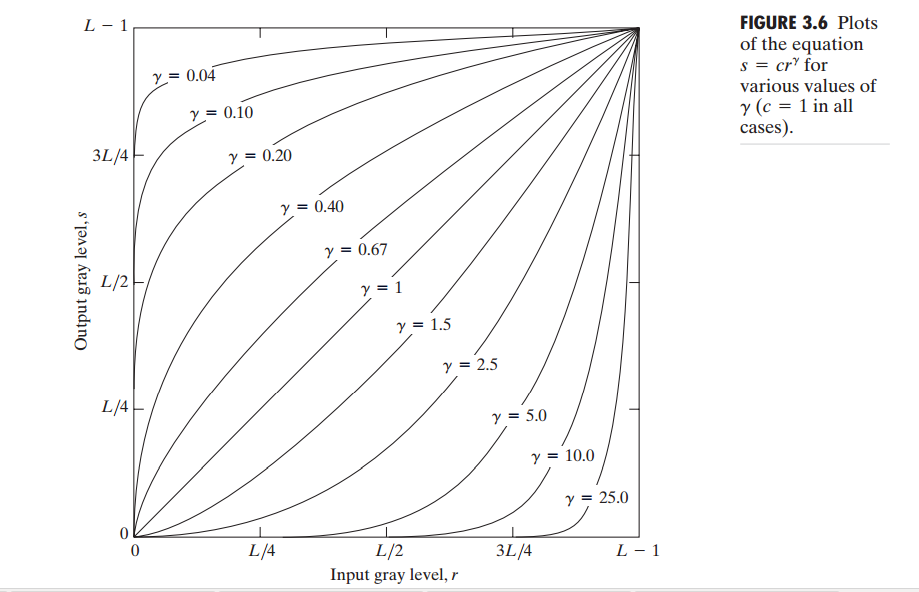
\includegraphics[width=300px]{./Imgs/powerDiag.png}}
\caption{Plots of s versus r for various values of $\gamma$}
\label{fig:powerDiag}
\end{figure}

 One of the most important and useful applications of this transformation is \textbf{gamma correction} in which value ranges in an input image would be mapped to a more appropriate range for certain image displayers to generate fitter images. The value of $\gamma$ in different applications corresponds to the using device and its properties. In fig\ref{fig:gamma0.4} in gamma correction process is $\gamma = 0.4$.\\
 Note that,  varying the value of gamma correction changes not only the brightness, but also the ratios of red to green to blue.\\
 
 \begin{figure}
 \center
 \makebox[\textwidth]{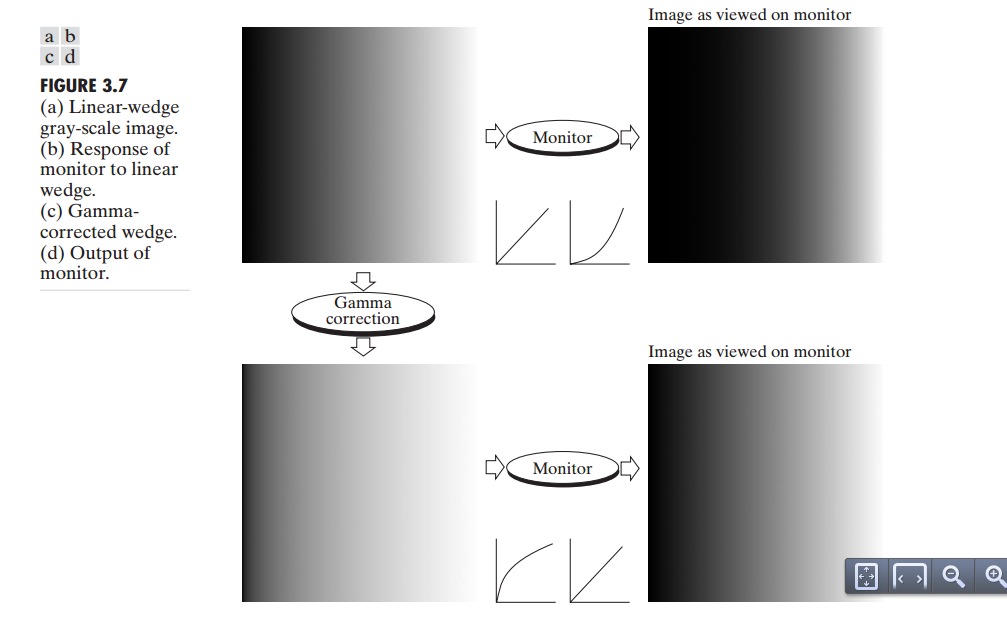
\includegraphics[width = 300px]{./Imgs/powerLaw.png}}
 \caption{Power-Law Transformation result and effect on an input image}
 \label{fig:gamma0.4}
 \end{figure}


 Note that, power-law transformation also affects image's contrast. Fig\ref{fig:powerLawContrast} illustrate the effect of this transformation on image's contrast. In this picture, the value of $\gamma$ increases in each case.
 
 \begin{figure}
 \center
 \makebox[\textwidth]{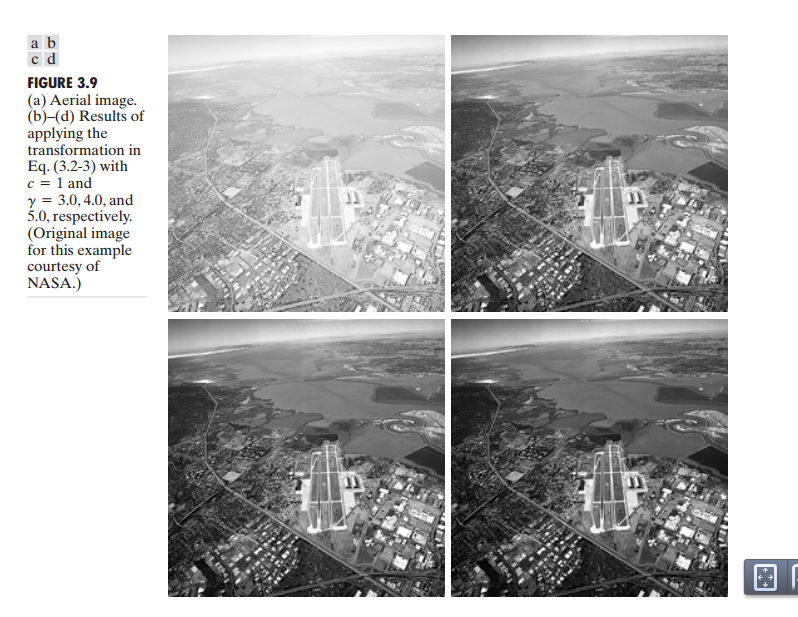
\includegraphics[width=300px]{./Imgs/powerLawContrast.png}}
 \caption{An illustration of power-law transformation's effect on image contrast.}
 \label{fig:powerLawContrast}
 \end{figure}
 
 
 \item [Piecewise-Linear Transformation Functions] This kind of transformation, fragments a transformation range to several subtransformations each specified in a disjoint range of overall transformation's definition range. Thus in each subtransformation any of above-mentioned transformations are applicable. Event though, this method provides us a great opportunity to make more complex and more advantageous transformations, it needs more user input.\\
 There are some examples of this method's applications.
 \begin{description}
 \item [Contrast Stretching] Creating a transformation function which is partially defined for different ranges for $(r,s)$ pairs. Fig\ref{fig:[pieceWiseContrast} demonstrates such an example function.
 \begin{figure}
 \center
 \makebox[\textwidth]{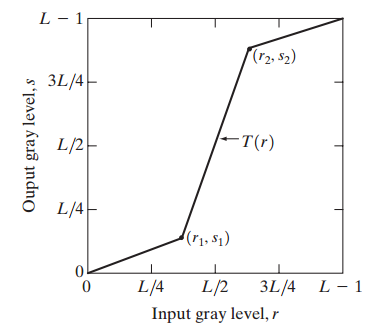
\includegraphics[width=200px]{./Imgs/pieceWiseContrast.png}}
 \caption{An example of piecewise-transformation function for contrast stretching.}
 \label{fig:[pieceWiseContrast}
 \end{figure}
 
 \item[Gray-Level Slicing] This kind of transformation is widely used in making a specified gray-level range of input image more salience. 
 
 \item[Bit-Plane Slicing] Separating bit planes of an image can make worthwhile contribution in achieving better results in applications. Fig\ref{fig:bitPlaneSlicing} displays application of such transformation on an input image of a fractal.
\begin{figure}
\center
\makebox[\textwidth]{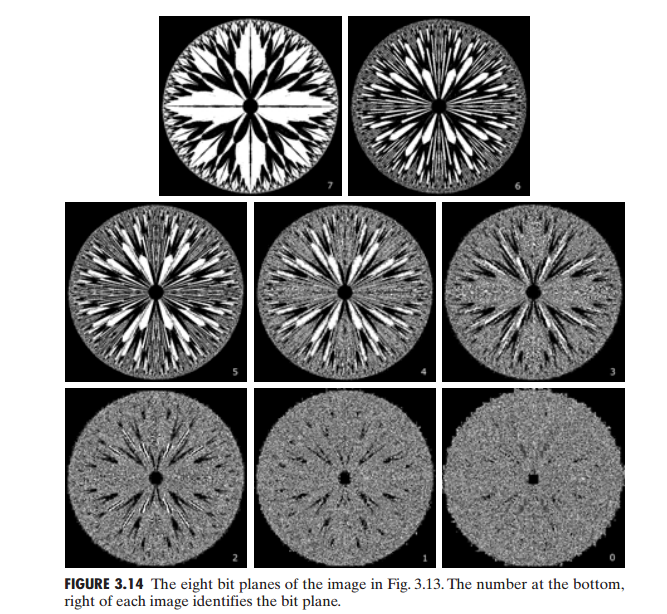
\includegraphics[width=300px]{./Imgs/bitPlaneSlicing.png}}
\caption{Applying a bit-plane slicing transformation on bit planes of a fractal image in order to separate bit-planes.}
\label{fig:bitPlaneSlicing}
\end{figure} 
 
 \end{description}
 
 
 \end{description}
%--------------------------------------------------------------------
\section{Histogram Processing}
\begin{description}
\item [Definition] A histogram of a gray level image with gray level range $[0, L-1]$ is a function $h(r_k) = n_k$ where $r_k$ is $k$th gray level and $n_k$ is the number of pixels with gray level $r_k$. Note that normalization gives an estimate of the probability of a pixel having gray level $r_k$, as follows:
\begin{center}
$P(r_k) = \frac{n_k}{n}.$
\end{center}

\item [Histogram Equalization] We define a transformation in following format:
\begin{center}
$s = T(r)$
\end{center}
Where $r$ is the gray level of a pixel, $s$ is a new gray level for pixel and $T(.)$ is a transformation function satisfying following conditions:
\begin{enumerate}
\item [a] Is \textit{monotonically increasing} in range $[0, 1]$ and is \textit{single\_vaued}
\item [b] $0 \leq T(r) \leq 1$ for $0 \leq r \leq 1$
\end{enumerate}
	\begin{description}
	\item[Theorem] Taking two random variables $r$ and $s$, given their probability density functions  $p_r$ and $p_s$, where $s = T(r)$, with known transformation function $T$ satisfying conditions (a) and (b), where $T^{-1}$ satisfies condition (a), $p_s$ can be obtained simply from formula:
	\begin{center}
	$p_s = p_r \cdot \abs{\frac{dr}{ds}}$
	\end{center}
	\item [Histogram Smoothing]
	Taking \textit{cumulative density function (CDF)} as transformation function, gives a transformation $T$ smoothing the histogram of an image:
	\begin{center}
	$
	s = T(r) = CDF_r = \int_0^rp_r(\omega) d\omega 	
	$\\ 
	$
	\frac{ds}{dr} = \frac{dT}{dr} = \frac{d\int_0^r p_r(\omega) d\omega}{dr} = \frac{p_r}{dr}
	$\\
	$
	p_s = p_r \cdot |\frac{dr}{ds}| \Rightarrow p_s = p_r \cdot |\frac{1}{\frac{ds}{dr}}| = p_r \cdot |\frac{1}{p_r}| = 1
	$\\
	$
	p_s = 1 \Rightarrow s $ is drawn from a $uniform$ distribution
	\end{center}
	\end{description}
\item [Histogram Matching (Specification)] The method used to generate image having a \textit{specific histogram shape} is called histogram matching.\\
Assume the given image's gray level is denoted by $r$ and the specific gray level that we would achieve on processed image is denoted by $z$.\\
	Given:
	\begin{center}
	$p_r$ and $p_z$ for input and desired output image.
	\end{center}
	Define:
	\begin{center}
	$G(z) = \int_0^s p_s(\omega) d\omega = s$
	\end{center}
	From before, we have:
	\begin{center}
	$s = T(r) = \int_0^r p_r(\theta) d\theta$
	\end{center}
	Thus:
	\begin{center}
	$G(z) = \int_0^s p_s(\omega) d\omega  = \int_0^r p_r(\theta) d\theta = s = T(r)$
	\end{center}
	Therefore:
	\begin{center}
	$z = G^{-1}(s) = G^{-1}(T(r))$
	\end{center}
	Note that: $G$ is computable given $p_z$ and then if $G^{-1}(z)$ exists, it can be computed by above-mentioned equation.
	\begin{description}
	\item [Implementation in discrete mode] Denote each set of gray levels by $\{r_j\}$, $\{s_j\}$ and $\{z_j\}$, where $j = 0, 1,\cdots, L-1$.\\
	Assume that $T(r)$ is a transformation function demonstrated by a table specifying the value of $s_i$ for $r_i$ directly. By applying this transformation, histogram-equalized image can be obtained. Also, given $p_z$ we can compute $G(z)$ as a transformation function by computing \textit{CDF} of $p_z$. Correspondingly, given each $v_i = G(z_i)$ we can compute $z_i = G^{-1}(v_i)$ having transformation function $G(z)$. According to definitions, $v = s$, so we can compute $z_i$ using this process for each $r_i$ of input image's gray levels. This final transformation, also, could be implemented using a table. Having this final transformation table, we can obtain each final value $z_i$ for each input $r_i$ directly and generate corresponding \textit{histogram-specified} output image.
	\end{description}
\end{description}

%--------------------------------------------------------------------
\section{Local Enhancement}
Although this global approach is suitable for overall enhancement, there are cases in which it is necessary to enhance details over small areas in an image. The histogram processing techniques previously described are easily adaptable to local enhancement. The procedure is to define a square or rectangular neighborhood and move the center of this area from pixel to pixel. At each location, the histogram of the points in the neighborhood is computed and either a histogram equalization or histogram specification transformation function is obtained. This function is finally used to map the gray level of the pixel centered in the neighborhood.
%---------------------------------------------------------------------
\section{Arithmetic/Logic Operations on Images}
This operations are applicable on two or more images, e.g. subtraction. In the case of login operations, pixels are considered as a string of binary numbers (values of bits of pixels).\\
\begin{description}
\item[Masking] or \textit{Region of Interest (ROI) processing}, is the process of applying \textit{AND} or \textit{OR} logic operators on an image. It is used to isolate an area for processing.\\
\item[Multiplication] can be used as a more effective method to create a grey-level masked image rather than binary one.
\item[Image Subtraction] 
	The formulation is as follows:
	\begin{equation}
		s(x, y) = f(x, y) - g(x, y)
	\end{equation}
	where $s$ is the subtraction result of images $f$ and $g$.
\begin{description}
	\item[Mask Mode Radiography] In this method, a picture of target texture of patient's body has been taken first, then after injecting a special medium into bloodstream, another picture of the same region has been taken. Subtraction of these two pictures, yields a clear picture of arteries in the target texture. 
	\begin{figure}[h]
	\centering
	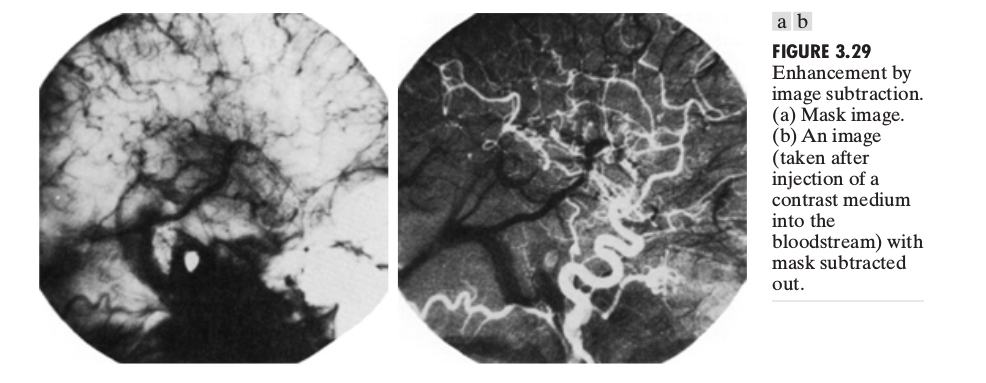
\includegraphics[width=300px]{./Imgs/mmr.png}
	\caption{MMR; extracting picture of arteries by subtraction}
	\end{figure}
\end{description} 
Note that there exist two normalization methods after subtraction:\\
\begin{enumerate}
	\item Add 255 to every pixel and divide all pixels by 2.
	\item Find min and max pixel values and transform values to be in range of [0-255].
\end{enumerate}

\item[Image Averaging]

\end{description}





%----------------------------------------------------------------------------------------
%	BIBLIOGRAPHY
%----------------------------------------------------------------------------------------

\bibliographystyle{apalike}

\bibliography{sample}

%----------------------------------------------------------------------------------------


\end{document}